\section{Background}
\begin{frame}
	\frametitle{NTCL}
	% Introducing NTCL, why and what it is
	\begin{itemize}
	\item Hardware independent frontend
	\item Hardware dependent backend
	\item Simplifying porting to different machines
	\item Access to NTCL: \url{gitlab.com/ntcl/ntcl}
	\item Examples: \url{github.com/thundermoose/NUCLEI-presentation-ntcl-examples}
	\end{itemize}
\end{frame}
\begin{frame}
\frametitle{Structure of NTCL}
\begin{center}
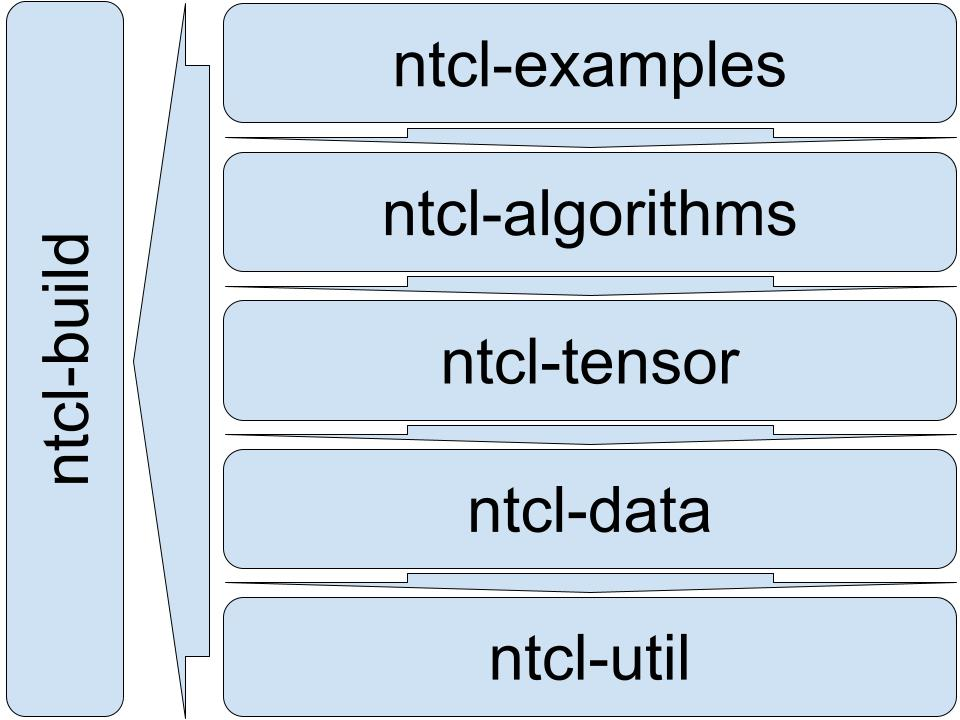
\includegraphics[scale=0.25]{figures/ntcl-repos.jpg}
\end{center}
\end{frame}
\section{Example replacing dgemm}
\begin{frame}[fragile]
	\frametitle{Example: gemm interface}
	\begin{lstlisting}
    real(real64), dimension(10,10) :: A
    real(real64), dimension(10,10) :: B
    real(real64), dimension(10,10) :: C
    ! Popluate arrays with random values
    call random_number(A)
    call random_number(B)
    C(:,:) = 0.0
    ! Perform a matrix-matrix multiplication 
    ! using BLAS dgemm
    call dgemm('N', 'N', 10, 10, 10, 1.0D0, A, &
               10, B, 10, 0.0D0, C, m)
	\end{lstlisting}
\end{frame}

\begin{frame}[fragile]
	\frametitle{Example: gemm interface}
	\begin{lstlisting}
    use :: algorithms_initializer, only : &
           algorithms_initialize, &
           algorithms_finalize
    use :: algorithms_api, only : &
           dgemm=>ntcl_gemm_real64
	\end{lstlisting}
\end{frame}

\begin{frame}[fragile]
	\frametitle{Example: gemm interface}
	\begin{lstlisting}
    call algorithms_initialize()
    ! Popluate arrays with random values
    call random_number(A)
    call random_number(B)
    C(:,:) = 0.0
    ! Perform a matrix-matrix multiplication 
    ! using BLAS dgemm
    call dgemm('N', 'N', 10, 10, 10, 1.0D0, A, &
               10, B, 10, 0.0D0, C, m)
    call algorithms_finalize()
	\end{lstlisting}
\end{frame}

\begin{frame}[fragile]
	\frametitle{Example: easy-contraction interface, Version 1}
	\begin{lstlisting}
    use :: algorithms_api, only : contract
    real(real64), dimension(m,k) :: A
    real(real64), dimension(k,n) :: B
    real(real64), dimension(m,n) :: C

    call random_number(A)
    call random_number(B)
    C(:,:) = 0.0

    call contract(C,A,B,'C(a,b)=A(a,c)*B(c,b)')
	\end{lstlisting}
\end{frame}


\begin{frame}[fragile]
	\frametitle{Example: NTCL-tensors}
\begin{lstlisting}
    real(real64), dimension(m,k) :: A
    real(real64), dimension(k,n) :: B
    real(real64), dimension(m,n) :: C
    ! ...
    call random_number(A)
    call random_number(B)
    C(:,:) = 0.0
\end{lstlisting}
\end{frame}

\begin{frame}[fragile]
	\frametitle{Example: NTCL-tensors}
\begin{lstlisting}
    use :: tensor_api, only: tensor
    ! ...
    class(tensor), allocatable :: tensor_A, tensor_B, tensor_C
    ! ...
    ! Copying tensors to GPU
    call allocate_and_copy_tensor(tensor_A, A)
    call allocate_and_copy_tensor(tensor_B, B)
    call allocate_and_copy_tensor(tensor_C, C)
\end{lstlisting}
\end{frame}

\begin{frame}[fragile]

\begin{lstlisting}
    use :: algorithms_api, only : &
            tensor_contraction, tensor_contraction_factory
    ! ...
    class(tensor_contraction) :: contraction
    ! ...
    ! Setting up the tensor contraction
    call tensor_contraction_factory%create(my_contraction, &
                                       'C(a,b)=A(a,c)*B(c,b)')
    ! Performing tensor contraction on GPU
    call my_contraction%contract(tensor_C, tensor_A, tensor_B)
\end{lstlisting}
\end{frame}

\begin{frame}
\frametitle{Benchmark on Frontier}
\begin{center}
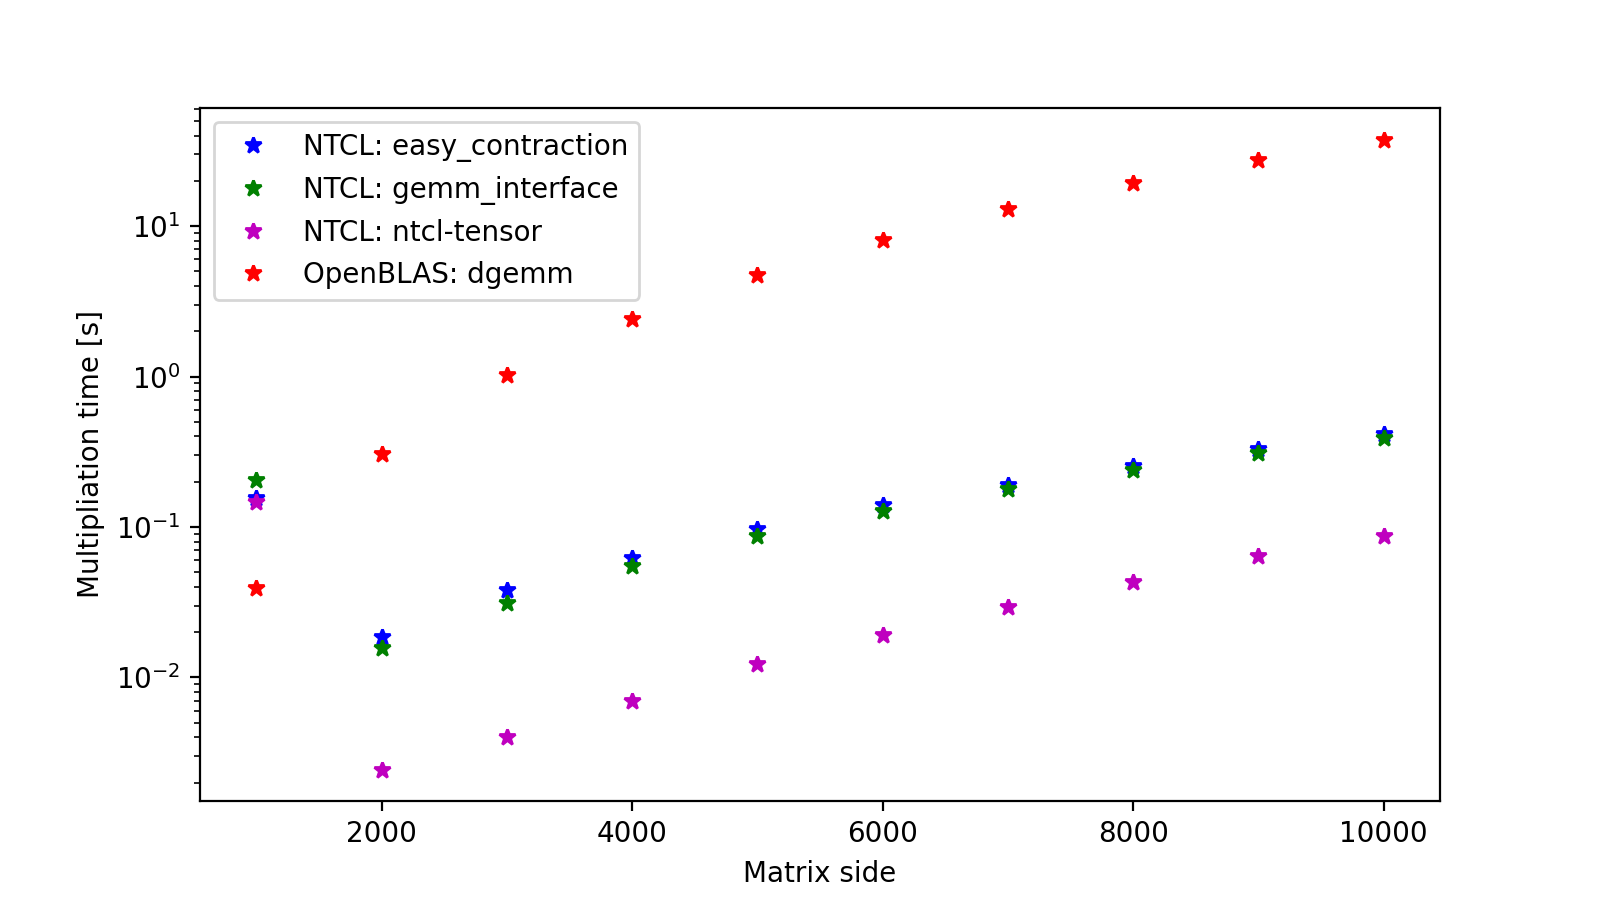
\includegraphics[scale=0.6]{figures/NTCL-vs-OpenBLAS-Frontier-matrix-multiplication.png}
\end{center}
\end{frame}

\begin{frame}
\frametitle{Benchmark on Frontier}
\begin{center}
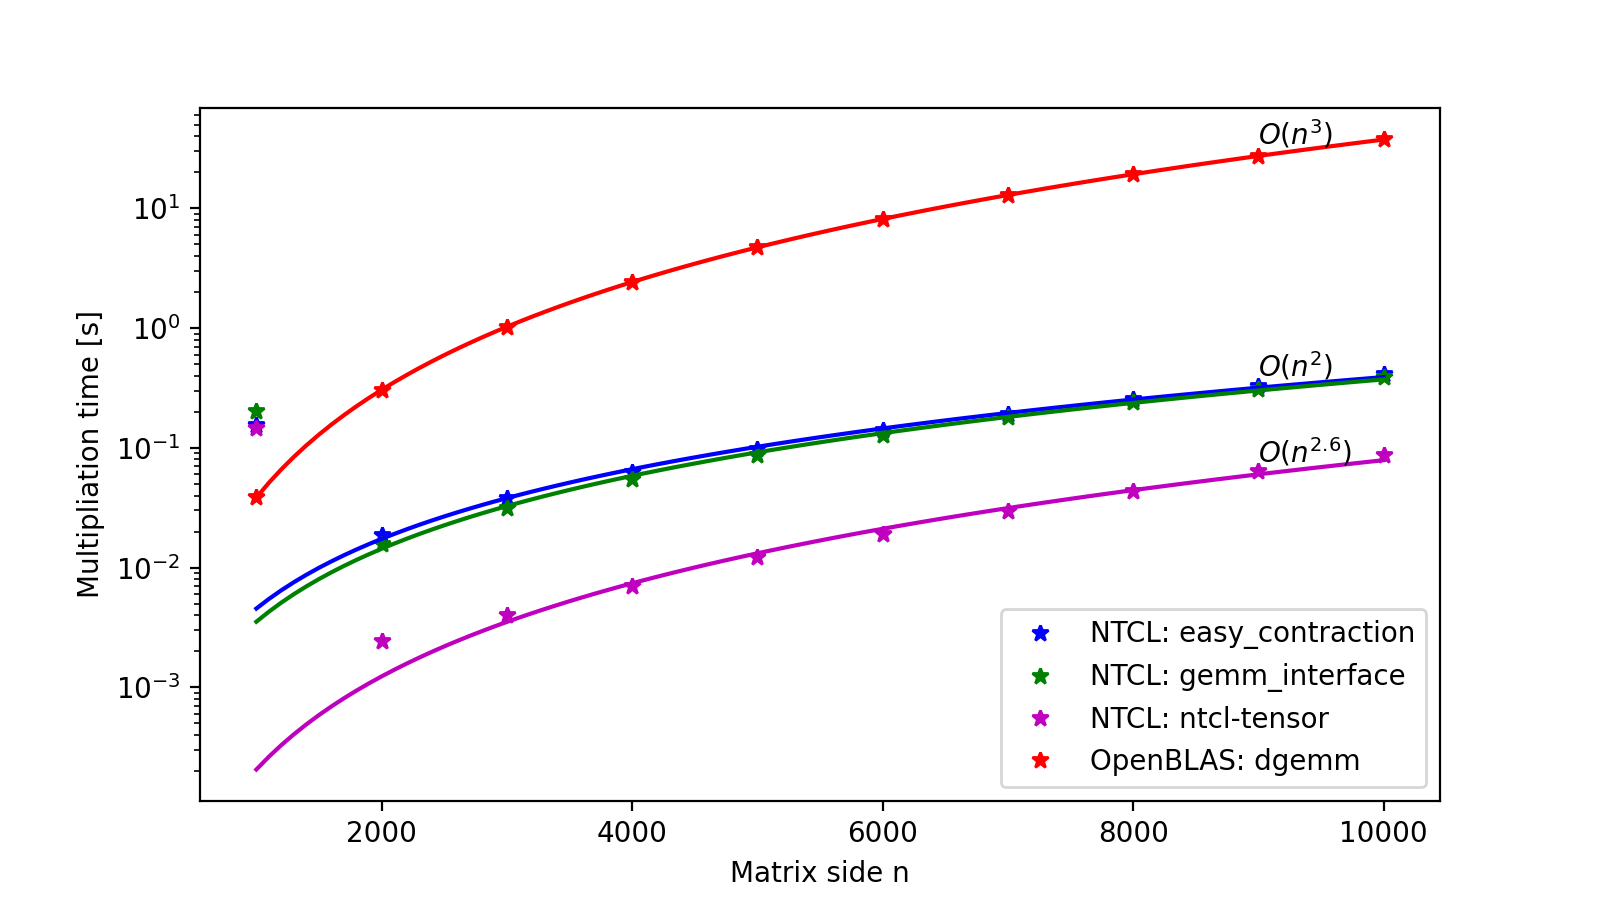
\includegraphics[scale=0.6]{figures/NTCL-vs-OpenBLAS-Frontier-matrix-multiplication-polyfits.png}
\end{center}
\end{frame}

\begin{frame}
\frametitle{Summary}
\begin{itemize}
\item NTCL provides a simple to use interface for GPU powered tensor operations
\item It allows you to port existing code using dgemm easily
\item Using Einstein summation notation wrting complicated tensor contractions is easy
\item NTCL is available to download at \url{gitlab.com/ntcl/ntcl}
\item NTCL examples can be found at \url{github.com/thundermoose/NUCLEI-presentation-ntcl-examples} 
\end{itemize}
\end{frame}

